\begin{figure}[t]
	\centering
		\begin{subfigure}{\columnwidth}
			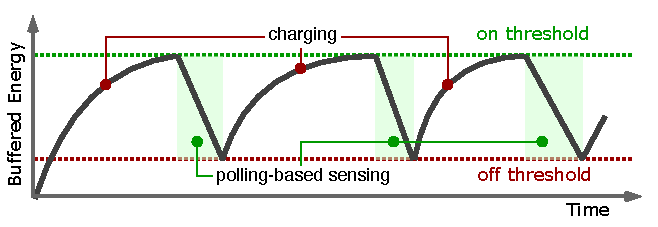
\includegraphics[width=\columnwidth]{figures/PowerCycleIntermittentSystem}
			\caption{When \sys does polling-based sensing, its energy consumption profile has, generally, two distinct rates: zero when it is charging, and a maximum when it is sensing.}
			\label{fig:pollingBasedSensing}
	\end{subfigure}
	\begin{subfigure}{\columnwidth}
		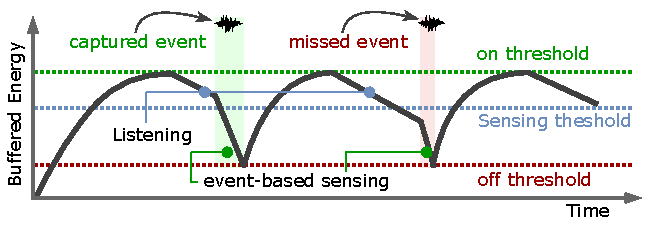
\includegraphics[width=\columnwidth]{figures/PowerCycleIntermittentSensor}
		\caption{When \sys does event-based sensing, it stays in low-power mode waiting for an external event to wake up the node. Consequently,  it has three distinct energy consumption rates: zero when it is charging, a maximum when it is sensing, and an in-between when it is sleeping. In favorable energy conditions, the sleeping mode may cause intermittent nodes to synchronize their power cycles on external events and miss the next ones.}
		\label{fig:eventBasedSensing}
\end{subfigure}
		\caption{\fullsys (\sys) energy profile for different sensing strategies. Green bars highlight successful sensing operations  while the red bar shows a failed sensing attempt due to insufficient buffered energy.}
		\label{fig:cisPwrCycle}
\end{figure} 
%
The \fullsys (\sys) is the abstraction of a group of battery-less intermittent sensor nodes seeking to provide continuous availability to the user. The key to success is to exploit the properties (i.e.\ randomness) of the ambient energy source to arrive at a uniform spreading of the awake times of the individual senor nodes to achieve the maximum coalesced availability. To this end we will first analyze the energy-consumption life cycle of an intermittently-power node, as well as the joined availability of multiple nodes. Then we will point out a practical aspect that is often overlooked; when intermittent nodes operate in favorable ambient conditions, their uncorrelated behavior changes due to the extra energy leading to synchronized patterns that need to be scrambled by introducing artificial, controlled randomization.


%\sys seeks to offer continuous sensing despite relying on ambient energy: an unpredictable and marginal power source. 
%orchestrates its nodes power cycles using a distributed approach (instead of relying on a master powerful node to coordinate coalesced nodes activities). 
%\sys seeks maximum time span of its underlying coalesced nodes through a distributed approach instead of a master node that orchestrates coalesced nodes on/off cycles. 
%\textcolor{red}{\bf Stephan: maybe add a sentence to introduce the upcoming (sub)sections.}

\subsection{Energy consumption}
%
\todo{reevaluate the importance of this paragraph and its location accordingly}
An intermittent sensor has a limited energy budget per power cycle. When it is tasked with a polling-based sensing activity, its energy consumption, generally, switches between two levels: zero when charging and maximum when it activates its microcontroller for data acquisition and processing, see Figure~\ref{fig:pollingBasedSensing}. (Note that we assume that the microcontroller is the dominant energy consumer module of a node.) However, in event-based sensing, a node puts its microcontroller into low-power mode and waits (or listens) for an external event to wake up the microcontroller. In case of the command recognizer we exploit the microphone's wake-on-sound feature to send an interrupt to the microcontroller, which will then start recording the sound samples from the microphone. This hardware approach is most energy efficient, but can be mimicked in software by periodic polling (i.e.\ acquiring 1 sound sample and checking if it exceeds the acoustic noise floor). This wake-on-event style of operation is important as the minimal energy consumption during sleep significantly prolongs the period during which an event can be handled, see Figure~\ref{fig:eventBasedSensing}. Although in reality the sleep and active phases draw quite different levels of power (128 vs. 849~$\mu$W on our hardware, see Table~\ref{tab:power_usage}) we will model the life cycle of a sensor node simply as an on-period followed by an off-period (in which the node recharges its energy buffer) as that suffices to analyze the collective availability of a \sys.
%The idle listening mode, which is important for successful sensing, complicates the design of the \sys.

\subsection{Coalesced availability}
\label{subSec:availability}
%
\begin{figure}[t]
		\centering
		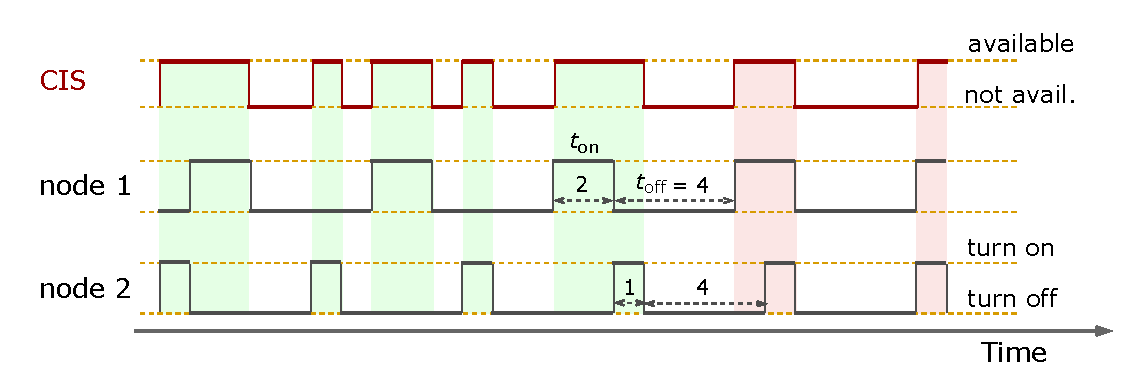
\includegraphics[width=\columnwidth]{figures/cisOntime}
		\caption{A \fullsys's availability is the emerging collective on-time of its intermittent nodes' on-times. The difference between the power cycles leads to a constant relative shift between the nodes duty cycles. This, in turn, causes their on-times to be uniformly distributed on the overall power cycle. The red bars indicate a minimum \sys time span---\sys's nodes are overlapping---whereas the green bars show the maximum time span of the \sys.}
		\label{fig:cisOntime}
\end{figure} 
%
\todo{Additional parameter: minimum time is needed to successfully capture an event. Nodes are uniformly distributed, and thus its overlapping intervals are also uniformly distributed. As such, for successful capturing, the overlapping interval must exceed the minimum time required for capturing an event. Another approach is to monitor the voltage level on the cost of additional hardware, complexity }

The \sys's on-time is the projection of its underlying intermittent nodes' on-times on the time axis. The \sys's on-time ranges from minimum (when all nodes on-times cluster together, see the red regions in Figure~\ref{fig:cisOntime}) to the maximum (when the overlapping between its nodes on-times is zero or when continuous availability is reached, highlighted with a green color in Figure~\ref{fig:cisOntime}). Two broad strategies for minimizing overlapping, hence, maximizing \sys availability, can be imagined: 
\begin{enumerate}[label=\roman*.]%[wide, labelwidth=!, labelindent=0pt]
%
		\item \textit{Explicit on-time division strategy}: Recent advancements in timing intermittent operations enable intermittent nodes to measure their on and off times with the help of an external ultra-low-power timer~\cite{hester2017timely}. Similar breakthroughs in passive communication enable ultra-low-power message exchange between battery-less nodes~\cite{li2015retro}. Intermittent nodes can use these advancements to apply a time-division multiplexing strategy to explicitly avoid overlapping on-times. For example, a node calculates its average on-time $\overline{t_{on}}$ and off-time $\overline{t_{\it off}}$ for $N$ power cycles. Then it measures the time difference between its power-up and the intended transmitting time $\Delta\,t$. Subsequently, it encodes the information $({\overline{t_{\it off}}, \overline{t_{on}}, \Delta\,t})$ in a message and broadcasts it. When a node receives this message it will have full knowledge about the transmitting node's power cycle. It can then alter its power cycle, relative to the transmitting nodes cycle, by either increasing (or decreasing) its power consumption to shorten (or lengthen) its on-time or shift its power cycle to a different time slot. This approach, obviously, assumes relatively stable nodes' power cycles. Assuming $N$ nodes observe the same on -and off- periods, the coalesced availability (their collective on-time) would be $N$ times the duty cycle of a node (or 100\% if the total length of the on-times exceeds a single power cycle).
%
\begin{figure}
		\centering
		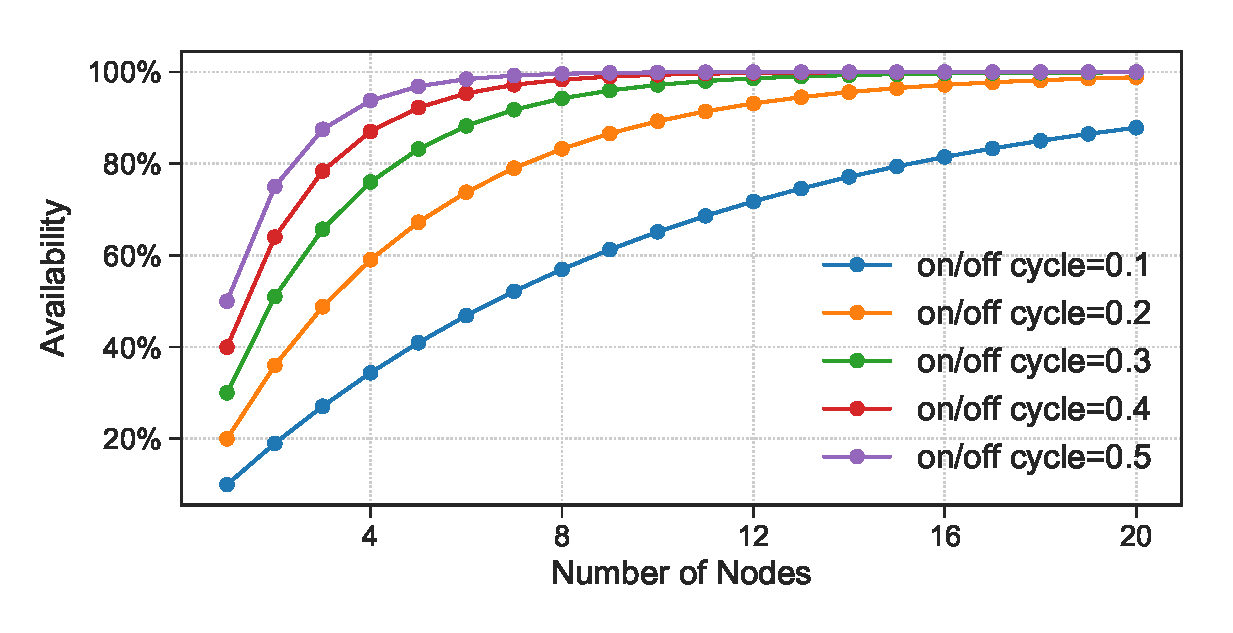
\includegraphics[width=\columnwidth]{figures/cisModel}
		\caption{\fullsys availability percentage for a different number of nodes and different duty cycles. The nodes are uniformly distributed and the \sys on-time evolves, when adding new nodes, according to the equation~\ref{eq:cisModel}.}
		\label{fig:cisModel}
\end{figure} 
%
		\item \textit{Implicit on-time division strategy}: With no information being exchanged between intermittent nodes, the best \sys can do is to uniformly distribute its node's on-times and maintaining this distribution over time. The key observation to uniformly distribute the nodes' on-times is to ensure that their power cycles are different. This can be achieved by forcing intermittent nodes to go into low-power mode upon power-ups. The length of this mode is randomly chosen for each node. This will change the length of the nodes on-times and, consequently, alter their power cycles. Figure~\ref{fig:cisOntime} shows the scenario of two intermittent nodes with different power cycles. Node 1 has a power cycle of 6 units of time and an on/off cycle of $\frac{1}{3}$. Node 2 has a power cycle of 5 units of time and an on/off cycle of $\frac{1}{5}$. Following the time axis from the left, we can see that the position of the on-time of Node 2 is shifted by 1 unit of time after each power cycle of Node 2. This implies that the on-times of the two nodes are $\frac{1}{3}$ of the time cluster together and $\frac{2}{3}$ of the time they are apart. If we extend the previous scenario to three or more nodes then the on-time of the resulting \sys can be described with the following formula,
				
\begin{equation}
	t_\text{on}(N) = t_\text{on}(N-1) + \frac{t_\text{off}(N-1)}{t_\text{off}(N-1)+t_\text{on}(N-1)} \times t_\text{on}(1),
		\label{eq:cisModel}
\end{equation}
where $N \in \mathbb{N}$ and  $t_\text{on}(N)$ is the on-time of a \sys with $N$ intermittent nodes. For the initial case where $N=1$ we define $t_\text{on}(0)\coloneqq 0$ and $t_\text{off}(0) \coloneqq 1$.
				
In addition to characterizing the availability of a \sys, equation~\ref{eq:cisModel} also states that the benefit of adding a node to the \sys is proportional to the \sys's off-time. In Figure~\ref{fig:cisModel} \sys availability percentage for different duty cycles and different number of intermittent nodes are shown.
\end{enumerate}
%s
\todo{this paragraph disconnect the paragraph below it from the one above it} There is a clear trade-off between the aforementioned methods. While the explicit control method provides fine control over the system 
distribution and therefore requires less number of nodes than the implicit control method, the implicit control method does not depend on the ability to communicate between the nodes and therefore it is simpler and more energy efficient. Since inter-node communication is beyond the capabilities of most of today's intermittent nodes, we focus on the implicit approach.
 
%Although the implicit method is relatively simple to implement and explore, the explicit control method is not a far-fetched idea considering the recent advancements in passive communication and intermittent timing. However, we opt to explore the implicit distribution control method as the hardware used to demonstrate the feasibility of passive light communication and ambient RF backscattering are not open source and re-making it is beyond the scope of this study.

\begin{figure}[t]
		\begin{subfigure}{\columnwidth}
			\centering
			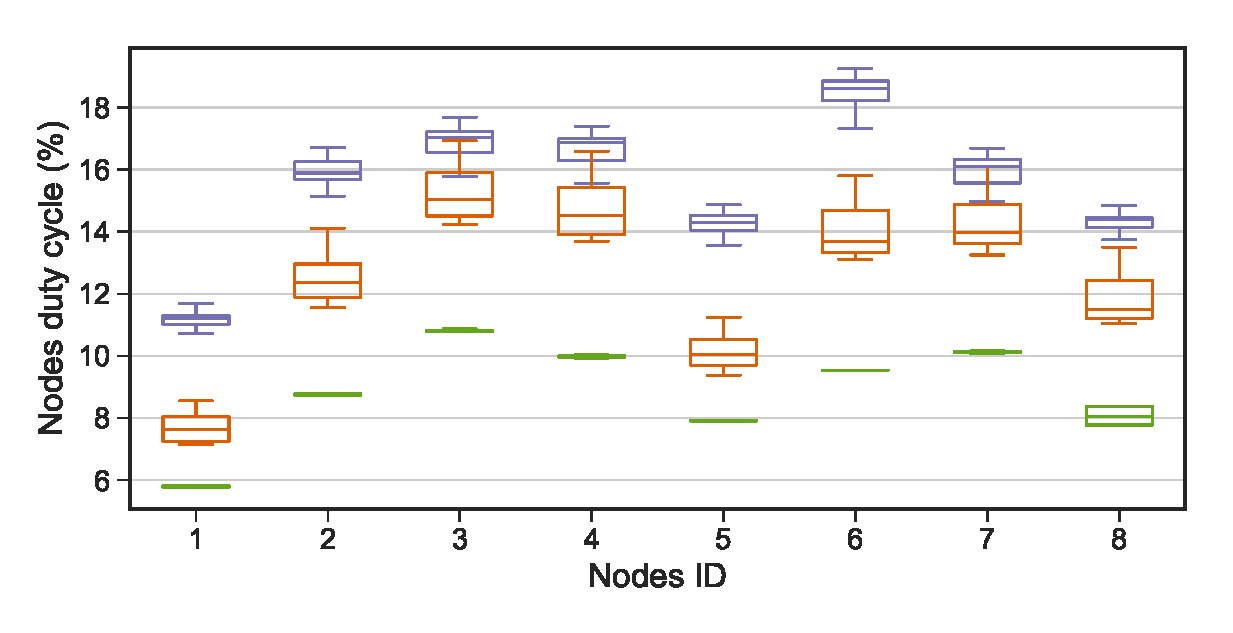
\includegraphics[width=\textwidth]{figures/natural_light_nodes_duty_cycles}
				\caption{light}
		\end{subfigure}\hfill
		\begin{subfigure}{\columnwidth}
			\centering
			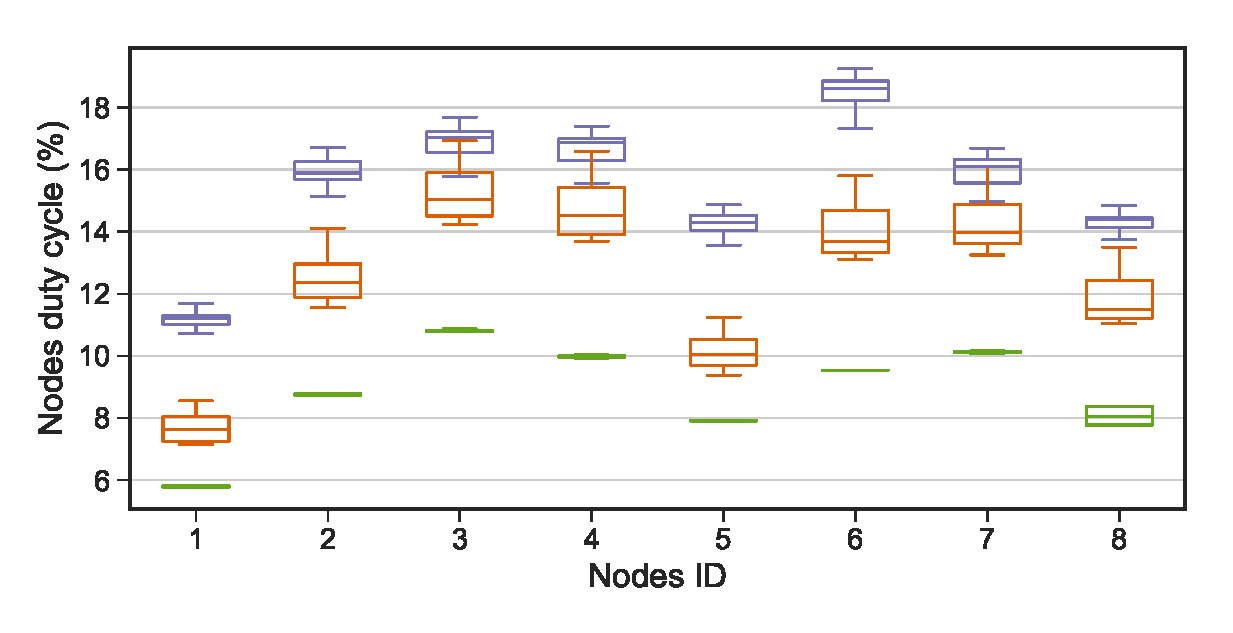
\includegraphics[width=\textwidth]{figures/natural_light_nodes_duty_cycles}
				\caption{\todo{correct the figures} RF}
		\end{subfigure}
		\caption{nodes's duty cycles are different for different energy conditions and different energy sources.}
		\label{fig:pwrCIS}
\end{figure} 

\paragraph{Implicit distribution of nodes' on-times}
Figure~\ref{fig:pwrCIS} shows the availability of \sys{}s when they are powered by different energy source and for a different number of intermittent nodes. We see that (i) the energy sources (sunlight, artificial light, and RF) power the \sys intermittently, (ii) the \sys availability increases with number of nodes, and (iii) this addition is proportional to the \sys off-time. 

The dashed lines represent Equation~\ref{eq:cisModel} expectation about the \sys availability for certain power cycles (10\% for the RF powered system, and 15\% for the light powered one). By comparing these lines to the measured ones we can conclude that these energy sources provide sufficient randomness to cause each node to have a slightly different power cycle which, in turn, causes their uptimes to be uniformly distributed in time.  


\subsection{Power States}
\label{sec:power_state}
A \sys can experience a wide range of ambient power intensities. For example, a solar-powered \sys may harvest no energy at night, modest energy from artificial light, and abundant energy from direct sunlight.  Generally, we can identify four different \sys powering states: 
\begin{itemize}
		\item \textit{Targeted power state}---These are the powering conditions that the \sys is designed for. In these  conditions, the \sys should work intermittently and have sufficiently randomized power cycles to uniformly distribute its intermittent nodes on-times and meet the desired availability percentage (Figure~\ref{fig:cisModel}). In general, the targeted powering conditions should be near worst energy harvesting conditions to ensure that the system is properly functioning for the majority of the time.
		\item \textit{Under-targeted power state}---Ultimately, the ambient energy is an uncontrollable power source, and it is not hard to imagine scenarios where a \sys will be under-powered or even comes to complete and long power down (for example, a solar \sys will come to a perpetual power down in the darkness). In general, for under-targeted energy conditions, the \sys behavior can be considered as undefined.
%
\begin{figure}
		\centering
		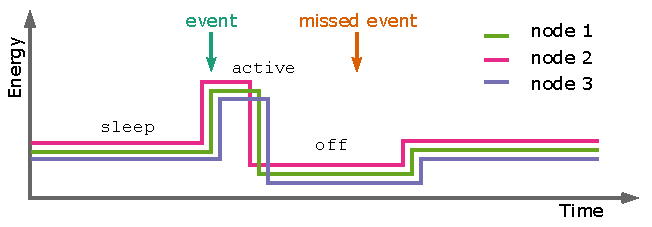
\includegraphics[width=\columnwidth]{figures/hibernating_power_state}
		\caption{\fullsys is in a hibernating power state when the energy harvesting rate approximates the energy consumption rate at the sleeping (or low-power) mode. In this state, the intermittent nodes lose the randomization in their power cycles. Thus, all the nodes capture the same event and power down shortly after missing the subsequent ones. Consequently, the \sys senses intermittently and does not take advantage of its redundant intermittent nodes to approach continuous sensing.}
		\label{fig:noRand}
\end{figure} 
%
		\item \label{it:hibernating} \textit{Hibernating power state}---In event-based sensing scenarios, the intermittent nodes of a \sys sleep in low-power mode waiting for an external event to wake them up. If the energy conditions are relatively higher than the targeted conditions, the nodes may not die and sustain their sleeping power consumption. This will cause them to synchronize their wake-ups on the first incoming event and their power down as the event capturing process depletes their energy buffers quickly. Consequently, the \sys may miss the next incoming events (specially if the events happens to arrive in bursts) causing it to sense intermittently instead of continuously, see Figure~\ref{fig:noRand}. 
		\item \label{it:continuous} \textit{Continuous power state}---Under direct mid-noon sun even a tiny solar panel can continuously power a sensor. In such conditions, the \sys will sense continuously without the need for randomization. Therefore, the job of a single node will be repeated $N$ times, and instead of sending a single message to a battery-powered or tethered sink---to push the data to the internet---$N$ identical messages will be sent which waste a lot of energy. 
				
\end{itemize}
%
\begin{figure}
		\centering
		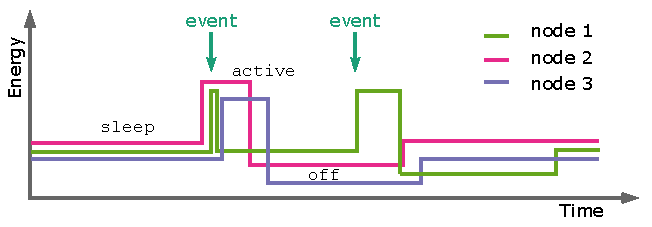
\includegraphics[width=\columnwidth]{figures/randomized_response}
		\caption{Randomized response helps in mitigating the hibernate-power-state problem. Also, it reduces the number of duplicated captured events when the \sys is overpowered. However, effective randomization strategy must be energy aware.}
		\label{fig:rand}
\end{figure} 

The inefficiencies highlighted in the hibernating and continuous power states can be mitigated by enforcing randomization on the response of intermittent nodes (Figure~\ref{fig:rand}): when a node is woken up by an external event it responds to that event with a certain probability. However, if the randomized response is enforced all the time, then the \sys will have a lower probability of catching events during the targeted energy conditions. Therefore, the \sys has to distinguish between the targeted and above-targeted energy conditions and randomize its response only during the hibernating and continuous power states. 


Choosing a fix response probability is an inefficient way of dealing with the over-powering problem as the number of active intermittent nodes at a given moment is a function of the total number of intermittent nodes and the power intensity at that time. Therefore, efficient randomization requires intermittent nodes to estimate the number of active nodes at the moment of an external event arrival (which is discuss it next) and respond proportionally.


\subsection{Intermittent Timing}
\label{subsec:interTimer}
%
\begin{figure}[t]
		\centering
		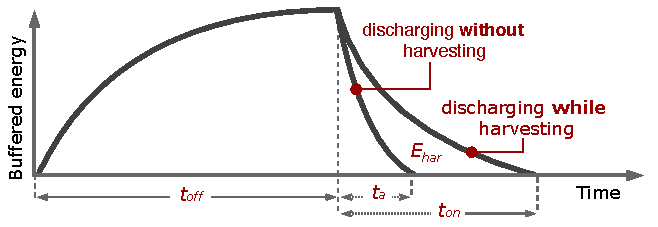
\includegraphics[width=\columnwidth]{figures/softwareClock}
		\caption{....}
		\label{fig:softwareClock}
\end{figure} 
%

Timing is a key building block of sensing systems. However, it is missing on intermittent nodes unless an additional dedicated timer circuit is added to them~\cite{hester2017timely}. Here we would like to propose an alternative way that does not require additional timer hardware. Obviously, the on-time of an intermittent node can be measured using the microcontroller's built-in timers. However, the difficulty is \textit{how an intermittent node can time its own off-time?}. Actually, answering this question does not only enable timing on intermittent devices but also enables them to estimate the richness of the ambient energy. 

\paragraph{Timing the death} 
Algorithm~\ref{algo:offTime} shows how a node can estimate its off-time. The basic idea is that a node measures its on-time while harvesting (Line~\ref{lin:ontime}) and compares it to the time required to drain the super capacitor without charging. The additional on-time $\Delta{t}$ is the result of the energy accumulated while executing. (Line~\ref{lin:deltat}). By assuming a relatively stable charging rate, a node can calculate how long it will be off charging (Line~\ref{lin:ehar}-\ref{lin:offtime}). Obviously, in order for the time estimation to be correct, the reference time and the on-time measurement must be done with same load ($a$). %\textcolor{red}{\bf Stephan: not sure what is meant here with "with same load"??/}
% off-time estimation 
\begin{algorithm}[t]
	\captionof{algorithm}{off-time estimation}
    \label{algo:offTime}
    \small
    \begin{algorithmic}[1]
		\State \Call{$f_\text{reboot}$}{$u$} $= u{+}{+}$ \Comment{power reboot counter}
		\State $i \leftarrow $ \Call{$f_\text{reboot}$}{$i$} \Comment{$i$ is a persistent variable}
		\State $E_\text{buf}$ \Comment{Size of energy buffer}
		\State $t_a$ \Comment{time of discharging $E_\text{buf}$ at load $a$, no harvesting}
		\State$ t_{i} \leftarrow x $ \Comment{timing every $x$ power cycles}
		%
		\If{$(i\mod t_{i})=0$}
		    \State $i=0$
			\State \Call{$f_\text{load}$}{$a$} \Comment{set node load to $a$ }
			\State \label{lin:ontime} $t_\text{on} \leftarrow$ \Call{$t_\text{pers}$}{\null} \Comment{persistent infinite loop}
		\EndIf
		\If{$i=0$}
			\State \label{lin:deltat}$\Delta{t} = t_\text{on}-t_a$  \Comment{time difference due to charging}
			\State \label{lin:ehar}$E_\text{har} \leftarrow (E_\text{buf}\div t_a)\times\Delta{t}$ \Comment{harvested energy}
			\State $P_\text{in} \leftarrow E_\text{har}\div{t_\text{on}}$ \Comment{incoming power}
			\State \label{lin:offtime}$t_\text{off} \leftarrow E_\text{buf}\div P_\text{in}$
		\EndIf
	\end{algorithmic}
\end{algorithm}

\subsection{Nodes overlapping}
\begin{figure}[t]
		\centering
		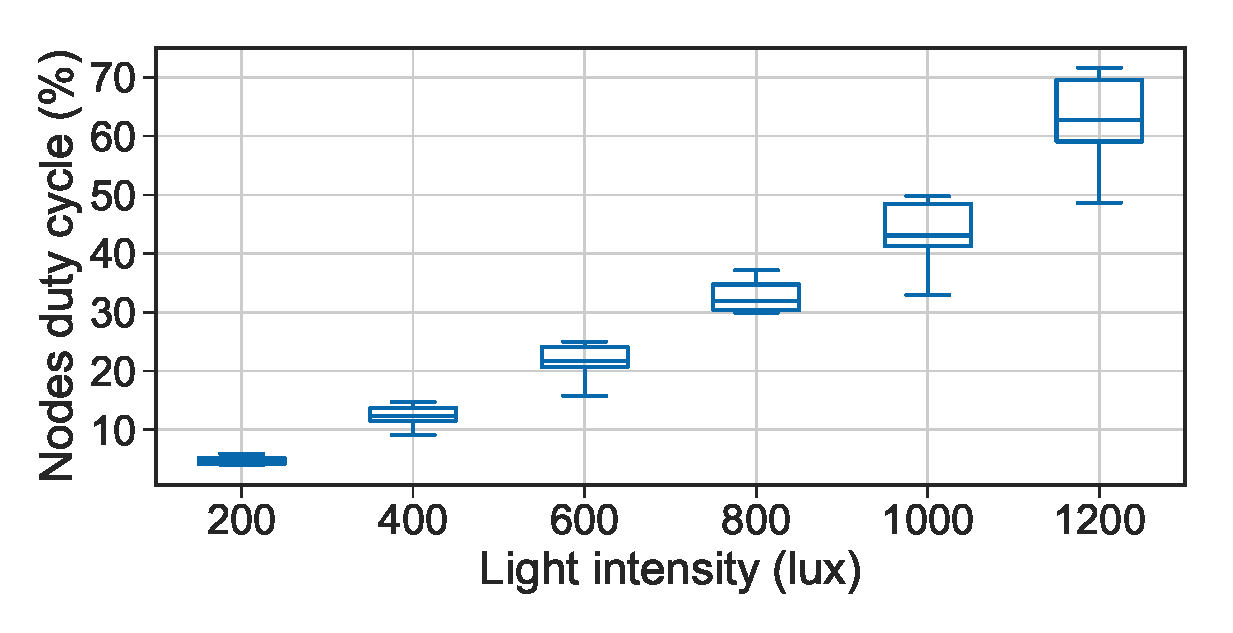
\includegraphics[width=\columnwidth]{figures/cis_dutyCycle.eps}
		\caption{The average duty cycles of eight intermittently powered nodes for different light intensity. In general, an individual node's duty cycle is a good indicator of the average duty cycle of its \sys.}
		\label{fig:cis_nodes_dutyCycle}
\end{figure} 

\begin{table}
		\centering
		\caption{Measuring intermittent nodes overlapping of a \sys of 8 intermittent nodes for different light intensities.}
		\begin{tabular}{lll}
				\hline
				light intensity (lux) & mean & std    \\
				\hline
				300	                  & 1.01 & 0.85   \\
				500                   & 1.63 & 0.98   \\
				800                   & 2.88 & 1.50   \\
				1200                  & 5.05 & 1.08   \\
				\hline
		\end{tabular}
		\label{tab:clusters}
\end{table}


In order for a node to estimate the number of active nodes at a given moment, first, it has to know the total number of nodes ($N$) in its \sys, which we assume to be known to the nodes before deployment. Second, this analysis is built on the observation that a node's on-time is a good indicator about the on-times of other nodes in the \sys, see Figure~\ref{fig:cis_nodes_dutyCycle}. A node can measure its on-time $t_\text{on}$ and off-time $t_\text{off}$ using  Algorithm~\ref{algo:offTime} (or an external dedicated timer~\cite{hester2017timely}). Then, it can estimate the maximum time span ($t_\text{max}$) of its \sys, which is the total duration of the nodes' on-times when they are aligned next to each other, as follows
\begin{equation}
t_\text{max} = N\times t_\text{on}.
		\label{eq:max_time}
\end{equation}
Then, from Equation~\ref{eq:cisModel}, the node calculates the \sys expected on-time ($t_\text{on}(N)$). As we argued in Section~\ref{subSec:availability}, nodes on-times are uniformly distributed over the \sys power cycle. Thus, the overlapping on-time is also uniformly distributed over the \sys on-time. Then, a node can calculate the average number of active intermittent nodes $n_\text{active}$ using the following formula,
\begin{equation}
	n_\text{active} = t_\text{max} \div t_\text{on}(N).
	\label{eq:active}
\end{equation}
and choose the proper randomization factor. If a second event, however, happens shortly after the first one, a node needs to update $N$ as follows, 
$$
N = N - n_\text{active}-1
$$
the $-1$ is because the node itself decided not to react on the first event. 

Table~\ref{tab:clusters} shows the average number of overlaps of an 8-nodes \sys for different light intensities. These measurements validate that nodes overlapping time is uniformly distributed over the \sys on-time. For example, at $\SI{1200}{lux}$ an individual node of our \sys has a duty cycle of $\approx$\,62\%. If we multiply it by the number of nodes (Equation~\ref{eq:max_time}) we get about 500\%. Figure~\ref{fig:cisModel} indicates that a \sys with eight nodes of duty cycles above 50\% has near 100\% availability. From equation~\ref{eq:active}, we find that the expected number of clustered nodes is 5 which is what Table~\ref{tab:clusters} also shows. 

